\chapter{Background}
This chapter covers the background for the fundamental concepts in this work in order to provide a deeper understanding of the research area and prepare the reader for the discussion of related work and the explanation of implementation details.
We start with the topic of conceptual modeling in the context of software systems.
Then, we introduce the approach of \textit{domain-driven design}, which is followed by the description of the Java programming language and its application to this research.

\section{Conceptual modeling of software systems}
Conceptual modeling is an integral part of software construction.
In software engineering field the term "conceptual schema" is often associated with the world of relational database management systems (RDBMS).
A conceptual schema describes the structure of a database from a high-level perspective.
More specifically, it identifies the core concepts and classifies them into tables, which contain columns that stand for the attributes of a concept.
A conceptual schema does not include any internal details about a database.

\n

For example, in a banking system domain, the conceptual schema might describe concepts such as \textit{banking accounts and transactions}, as well as their relationship.
One common language for expressing conceptual schemas is UML.
Consider the banking example illustrated in the following UML class diagram:

\begin{figure}[H]\centering
    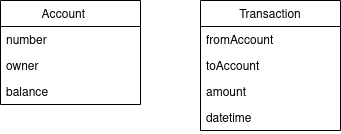
\includegraphics[scale=0.65]{images/banking.drawio.png}
    \caption{UML class diagram for a simplified banking domain}\label{fig:bank}
\end{figure}

Here the conceptual schema consists of two domain entities.
Both of them are characterized by specific attributes that describe their structure.
And it is a common occurence that the underlying structure of an entity might undergo some kind of modification.
For example, consider the diagram below that introduces a new attribute to the \texttt{Account} entity, namely, its creation date:

\begin{figure}[H]\centering
    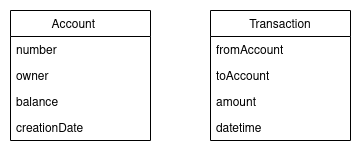
\includegraphics[scale=0.65]{images/banking1.drawio.png}
    \caption{UML class diagram illustrating an additive change to the conceptual model}\label{fig:bank1}
\end{figure}

\n

Modifications on a conceptual level, such as these, must be performed with caution, since they are fundamental in their nature.
This means that every part of the system that interacts with a modified concept should be taken into account during verification.
However, a simple additive change, as illustrated by the example, is relatively safe.
Consider another example showing an existing attribute of \texttt{Account} being modified:

\begin{figure}[H]\centering
    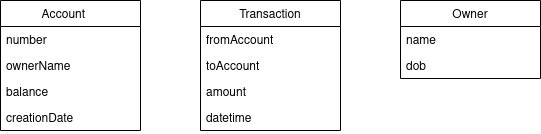
\includegraphics[scale=0.65]{images/banking2.drawio.png}
    \caption{UML class diagram illustrating a breaking change to the conceptual model}\label{fig:bank2}
\end{figure}

The \texttt{ownerName} attribute of \texttt{Account} has been replaced by \texttt{owner}.
The \texttt{Owner} concept has also been included in the diagram to provide the necessary context.
This kind of change is often refered to as a \textit{breaking change}, since it might "break" the system if any of its components were using the modified part.
Given that prior to this change the \texttt{ownerName} attribute was a simple textual representation, any part of the system that was refering to this attribute must be modified accordingly.
Ideally, after a modification has taken place, the system would be automatically validated to detect any errors that might have resulted from the modification.
In our example it would be expected that the validation mechanism reports that the \texttt{Account} concept does not define an attribute \texttt{ownerName}, if it was used prior to the modification.

%\n
%
%However, the world of software systems is not perfect.
%Database querying mechanisms work under the assumption that their input is consistent with the actual conceptual schema.
%If incorrect input is supplied, it will most likely cause the system to fail when it is already running or being tested.

\section{Domain-driven design and its terminology}
Domain-driven design, a term coined by Eric Evans \cite{ddd}, is an approach to conceptual modeling of a specific business domain.
Its main aim is construction of a domain model, which translates to a conceptual model of the domain.
At the heart of domain-driven design one of the basic building blocks is an \textit{entity}, that is, a domain object defined primarily by its identity.
We use the term \textit{entity} interchangeably with the term \textit{concept} assuming that the concept has an identity. 
Every entity is characterized (but not necessarily identified) by its \textit{properties} in the same way that every concept is characterized by its \textit{attributes}.

\section{Java programming language}
Java \cite{java} is a compiled, high-level, class-based, object-oriented programming language.
In practice it is often used to implement domain-driven software systems, mapping domain objects to Java classes.
Fields of a Java class are used to represent properties of an entity.
For example, the domain from \ref{fig:bank} could be modeled in the following way:

\begin{listing}[H]
    \begin{minted}{java}
        class Account {
            private int number;
            private String ownerName;
            private float balance;
        }

        class Transaction {
            private Account fromAccount;
            private Account toAccount;
            private float amount;
            private DateTime datetime;
        }
    \end{minted}
    \caption{The domain illustrated in \ref{fig:bank} modeled in Java.}
    \label{lst:bank}
\end{listing}

\section{Java reflection}
The reflection capabilities of Java are briefly discussed in this section, since they are often mentioned alongside with the terms \textit{metadata} and \textit{metaprogramming}.
In contrast with other compiled languages, such as C, Java is characterized by its sophisticated runtime mechanism that provides dynamic capabilities, such as reflection and code modification.
Reflection, in particular, makes metaprogramming possible, which allows the program to use other programs, itself included, as data.
For example, using reflection it is possible to obtain the type of a class field by its name:

\begin{minted}{java}
class Person {
    private Animal pet;
}

Person.class.getDeclaredField("pet").getType()); // class Animal
\end{minted}

Although this is a powerful programming technique that allows runtime type introspection to take place, it can not be used to treat the source code of a program as data at compile time.
The runtime nature of reflection indicates that reflection operates on objects constructed from compiled code.
This means that metadata obtained by using reflection exists only at runtime of the system, which is out of compiler's scope.

\section{Java annotations}
The Java Language Specification \cite{jls} defines a special construct – annotations – that provides data about a program that is not part of the program itself, in other words, it has no direct effect on the operation of code that is annotated.
Annotations may be used to provide additional information to the compiler or to be interpreted during runtime of the program.
We focus on the compile time processing of annotations.
As an example, the \texttt{@Deprecated} annotation can be used to tell the compiler to generate warnings in places where the annotated element is used.

\begin{minted}[escapeinside=||]{java}
class Transformer {
    @Deprecated
    public static boolean isTransformable(Item item) {
        ...
    }
}

// warn: the method Transformer.isTransformable(Item) is deprecated
Transformer.|\st{isTransformale}|(someItem);
\end{minted}

The annotated method can still be used as if there was no annotation, but the warning makes it clear to a software engineer that the method is no longer supported and its usage is discouraged.

\section{Annotation processing}
Annotation processing, as its name implies, is a mechanism for processing annotations in the source code at compile time.
An important distinction from the previously mentioned concept of reflection is that the input of an annotation processor is an AST\footnote{Abstract syntax tree is a tree-like data structure used by the compiler to represent the structure of program source code.} constructed from the source code.

\n

The \texttt{@Deprecated} annotation in the example above is one of the Java built-in annotations. It gets processed by a built-in annotation processor that is a part of the Java compiler.

\n

The standard library of Java includes a common interface to all annotation processors, so software engineers can provide their own implementations, and instruct the compiler to use them.
Apart from issuing compile time warnings and errors, annotation processing supports programmatic generation of new code.
The following figure depicts the compilation process of javac\footnote{Java compiler included in the JDK from Oracle}.

\begin{figure}[H]\centering
    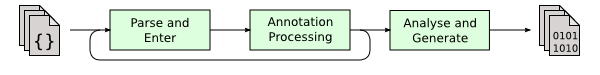
\includegraphics[scale=0.8]{images/javac-flow.png}
    \caption[Compilation process of javac]{Compilation process of \texttt{javac}}\label{fig:javac-flow}
\end{figure}

Java compilation process can be broken down into the following steps:

\begin{enumerate}
    \item The input source files are parsed to build a syntax tree.
    \item All appropriate annotation processors are run until no new files are generated.
    \item The syntax tree is analyzed to generate byte-code.
\end{enumerate}

It is important to mention that step 1 may differ across compiler implementations. The main difference lies in the input of a compiler. There is a notion of incremental compilation, which provides an ability to limit the number of source files that are passed as input to the compiler. As opposed to traditional compilation that requires the whole set of source files to be recompiled, an incremental compiler’s input is limited to that portion of the program that was modified.

\n

The built-in annotation processing API in Java has a rich collection of types that model the source language itself, equipping programmers with a powerful abstraction to analyze the syntax tree.\footnote{\texttt{javax.annotation.processing -- \url{https://docs.oracle.com/javase/8/docs/api/javax/annotation/processing/package-summary.html}}}
